\documentclass[12pt, a4paper, openright]{book}


\usepackage{amsmath}
\usepackage{graphicx}
\usepackage{hyperref}  % for citing URLs
\usepackage{listings}
\lstset{breaklines=true}
\pagestyle{plain}
\newcommand{\HRule}{\rule{\linewidth}{0.5mm}}

\topmargin       0in
\oddsidemargin   0in
\evensidemargin  0in
\headheight      0in
\headsep         0in
\topskip         0in
\textheight      9in
\textwidth       6.5in

\begin{document}

\frontmatter
\begin{titlepage}
\begin{center}

% Upper part of the page. The '~' is needed because \\
% only works if a paragraph has started.

\includegraphics[width=0.27\textheight]{iitbLogo}~\\[1cm]

\textsc{\LARGE IIT Bombay}\\[1.5cm]

\textsc{\Large Dual Degree project}\\[0.5cm]

% Title
\HRule \\[0.4cm]
{ \huge \bfseries Cognitive Radio using OpenBTS\\[0.4cm] }

\HRule \\[1.5cm]

% Author and supervisor
\begin{minipage}{0.4\textwidth}
\begin{flushleft} \large
\emph{Author:}\\
Swrangsar \textsc{Basumatary}
\end{flushleft}
\end{minipage}
\begin{minipage}{0.4\textwidth}
\begin{flushright} \large
\emph{Supervisor:} \\
Prof.~S~N \textsc{Merchant}
\end{flushright}
\end{minipage}

\vfill

% Bottom of the page
{\large \today}

\end{center}
\end{titlepage}

\begin{abstract}

The concept of interference temperature was introduced by the FCC as a new metric for quantifying and managing interference. Using this model, cognitive radios (CRs) operating in licensed frequency bands would be able to measure their current interference environment and adjust their transmission characteristics so as not to raise the interference temperature over a regulatory limit.

As of now it is hard to predict whether interference temperature is going to be practical because no one has been able to come up with a solution that is agreed upon by everyone. The research on interference temperature was abandoned by the Federal Communications Commission (FCC) in 2007 but there is some hope of a comeback.

This document highlights what I have learned about interference temperature as part of my supervised research exposition.

\end{abstract}


\setcounter{tocdepth}{2}
\tableofcontents

\setlength{\parindent}{0em}
\setlength{\parskip}{1em}
\setlength\arraycolsep{2pt}

\mainmatter
\chapter{Introduction}
\section{Background}
The electromagnetic radio spectrum is a natural resource that remains underutilized \cite{haykin05}. It is licensed by governments for use by transmitters and receivers. With the explosive proliferation of cell phones and other wireless communication devices, we cannot afford to waste our spectral resources anymore.

In November 2002, the Spectrum Policy Task Force, a group under the Federal Communications Commission(FCC) in the United States, published a report saying \cite{repFCC}, 
\begin{quote}
``In many bands, spectrum access is a more significant problem than physical scarcity of spectrum, in large part due to legacy command-and-control regulation that limits the ability of potential spectrum users to obtain such access.''
\end{quote}

If we were to scan the radio spectrum even in metropolitan places where it's heavily used, we would find that \cite{staple04} :
\begin{enumerate}
	\item some frequency bands are unoccupied most of the time,
	\item some are only partially occupied and
	\item the rest are heavily used.
\end{enumerate}

The underutilization of spectral resources leads us to think in terms of \emph{spectrum holes}, which is defined as \cite{kolodzy01}:
\begin{quote}
\emph{A spectrum hole is a band of frequencies assigned to a primary user, but, at a particular time and specific geographic location, the band is not being utilized by that user.
}
\end{quote}

Spectrum utilization can be improved significantly by allowing a secondary user (who is not being serviced) to use a spectrum hole unoccupied by the primary user at the right location and the time in question \cite{haykin05}. \emph{Cognitive Radio}, which is usually implemented using a software defined radio, has been proposed as the means to promote the efficient use of spectral resources.

\section{Cognitive Radio}



\section{Organization}

\chapter{Overview of traditional GSM networks}

\section{What is GSM?}
GSM, or Global System for Mobile Communications,  is a European standard for the Mobile telecommunications and it is considered as one of the most popular standard worldwide.There are thirteen different frequency bands de�ned in GSM. However, the 850 MHz, 900 MHz, 1800 MHz, and 1900 MHz bands are the most commonly used. The frequency bands employed within each of the four ranges are similarly organized. They differ essentially only in the frequencies, such that various synergy effects can be taken advantage of; hence we only give some details for the usage in the 900 MHz band.


In the 900 MHz band, a total of 70 MHz bandwidth is allocated, two 25-MHz frequency
bands for uplink and downlink and a 20 MHz unused guard band between them. The MS transmits
in the 890- to 915-MHz range (uplink) and the BTS transmits in the 935- to 960-MHz
(downlink) band. This corresponds to 124 duplex channels, where each channel within a BTS is
referred to as an Absolute Radio Frequency Channel Number (ARFCN). This number describes a pair of frequencies, one uplink and one downlink, and is given a channel index between C0 and C123, with C0 designated as the beacon channel. An ARFCN could be used to calculate the exact frequency (in MHz) of the radio channel. In the GSM 900 band, this is computed by the following equations:

\begin{align}
F_{uplink}(n) &= 890 + 0.2*n \qquad & 1\leq{}n\leq{}124 \nonumber\\
F_{downlink}(n) &=F_{uplink}(n) + 45  \qquad & 1\leq{}n\leq{}124 \nonumber
\end{align}

Similar formulas are also de�ned for the other GSM frequency bands.


The principle component groups of a GSM network are as follows:
\begin{itemize}
	\item The Mobile Station (MS)
	\item The Base Station System (BSS)
	\item The Network Switching System(NSS)
\end{itemize}

Diagram of GSM architecture
fig


\subsection{Mobile Station}
The MS consists of two parts, the Mobile Equipment (ME) and  Subscriber Identity module (SIM). The ME has an identity number called the International Mobile Equipment Identity (IMEI) associated with it, which is unique for that particular device and permanently stored in it.The SIM card consists the International Mobile Subscriber Identity(IMSI) number which is used to identify the subscriber to the system. The IMEI and IMSI are independent of each other and hence, allowing personal mobility.

\subsection{Base Station System}
The GSM Base Station System is the equipment located at a cell site. It comprises a combination of digital and RF equipment. The BSS provides the link between the MS and the Mobile Services Switching Centre (MSC).
The BSS consists mainly of:
\begin{description}
	\item[The Base Transceiver Station(BTS)]  
	The BTS contains the RF components that provide the air interface for a particular cell. This is the part of the GSM network which communicates with the MS. The antenna is included as part of the BTS.
	\item[The Base Station Controller(BSC)]  
	The BSC  provides the control for the BSS. The BSC communicates directly with the MSC. The BSC may control single or multiple BTSs. Crucial functions like radio channel link establishment, frequency hopping, and handovers from one cell to another.

\end{description}

\subsection{Network Switching Subsystem} The Network Switching System includes the main switching functions of the GSM network. It also contains the databases required for subscriber data and mobility management. Its main function is to manage communications between the GSM network and other telecommunications networks. The main components of the Network Switching System are: 
\begin{description}
	\item[Mobile Services Switching Centre(MSC)] The MSC does call-switching and its overall purpose is the same as that of any telephone exchange. When the MSC provides the interface between the PSTN and the BSSs in the GSM network it will be known as a Gateway MSC. In this position it will provide the switching required for all MS originated or terminated traffic. Each MSC provides service to MSs located within a defined geographic coverage area. One MSC is capable of supporting a regional capital with approximately one million inhabitants. 
The functions carried out by the MSC are: Call Processing, Operations and Maintenance Support, Internetwork Interworking and Billing
	\item[Home Location Register (HLR)] The HLR is a central database that contains details of each mobile phone subscriber that is authorized to use the GSM core network.The  IMSI�s of each SIMs act as primary key to each HLR record. Each MSISDN is also a primary key to the HLR record. The HLR data is stored for as long as a subscriber remains with the mobile phone operator.Data stored in HLR against each IMSI are, GSM services that the subscriber has requested ,GPRS settings to allow subscriber to access packet services,current location of subscriber etc
	\item[Visitor Location Register (VLR)] The VLR is a database of the subscribers who have roamed into the jurisdiction of the MSC which it serves. Each main base station in the network is served by exactly one VLR, hence a subscriber cannot be present in more than one VLR at a time.The data stored in the VLR has either been received from the HLR, or collected from the MS.Data stored include: IMSI (the subscriber's identity number), authentication data,MSISDN ,GSM services that the subscriber is allowed to access, The HLR address of the subscriber.

\end{description}

\section{Um Interface}
The Um interface is the air interface for the GSM mobile telephone standard. It is the interface between the MS and the BTS. It is called Um because it is the mobile analog to the U interface of ISDN. Um is defined in the GSM 04.xx and 05.xx series of specifications.


The layers of GSM are initially defined in GSM 04.01 Section 7 and roughly follow the OSI model. Um is defined in the lower three layers of the model.

\subsection{Physical Layer (L1)}
The Um physical layer is defined in the GSM 05.xx series of specifications, with the introduction and overview in GSM 05.01. For most channels, Um L1 transmits and receives 184-bit control frames or 260-bit vocoder frames over the radio interface in 148-bit bursts with one burst per timeslot. There are three sublayers:

\begin{description}
	\item[Radiomodem] This is the actual radio transceiver. GSM uses 8PSK modulation with 1 bit per symbol which produces a 13/48 MHz (270.833 kHz or 270.833 K symbols/second) symbol rate and a channel spacing of 200 kHz. Since adjacent channels overlap, the standard does not allow adjacent channels to be used in the same cell. The standard defines several bands ranging from 400 MHz to 1990 MHz.GSM is frequency duplexed, meaning that the network and MS transmit on different frequencies, allowing the BTS to transmit and receive at the same time. Transmission from the network to the MS is called �downlink" and from the MS to the network is called �uplink". GSM uplink and downlink bands are separated by 45 or 50 MHz. Uplink/downlink channel pairs are identified by an index called the ARFCN. Within the BTS, these ARFCNs are given arbitrary carrier indexes C0..Cn-1, with C0 designated as a Beacon Channel and always operated at constant power. The radio channel is time-multiplexed into 8 timeslots, each with a duration of 156.25 symbol periods. These 8 timeslots form a frame of 1,250 symbol periods. The capacity associated with a single timeslot on a single ARFCN is called a physical channel (PCH) and referred to as �CnTm" where n is a carrier index and m is a timeslot index (0-7).Each timeslot is occupied by a radio burst with a guard interval, two payload fields, tail bits, and a midamble.
	
	\item[Multiplexing and Timing] GSM uses TDMA to subdivide each radio channel into as many as 16 traffic channels or as many as 64 control channels. The multiplexing patterns are defined in GSM 05.02.Each physical channel is time-multiplexed into multiple logical channels according to the rules of GSM 05.02. Traffic channel multiplexing follows a 26-frame (0.12 second) cycle called a "multiframe". Control channels follow a 51-frame multiframe cycle. The C0T0 physical channel carries the synchronization channel(SCH), which encodes the timing state of the BTS to facilitate synchronization to the TDMA pattern.
	
	\item[FEC Coding] The coding sublayer provides forward error correction. As a general rule, each GSM channel uses a block parity code (usually a Fire code), a rate-1/2, 4th-order convolutional code and a 4-burst or 8-burst interleaver.

\end{description}

\subsection{Data Link Layer(L2)}
The Um data link layer, LAPDm, is defined in GSM 04.05 and 04.06. LAPDm is the mobile analog to ISDN's LAPD.

\subsection{Network layer(L3)}
The Um network layer is defined in GSM 04.07 and 04.08 and has three sublayers. A subscriber terminal must establish a connection in each sublayer before accessing the next higher sublayer.

\begin{description}
	\item[Radio Resource (RR)] This sublayer manages the assignment and release of logical channels on the radio.

	\item[Mobility Management (MM)] This sublayer authenticates users and tracks their movements from cell to cell. It is normally terminated in the VLR or HLR.

	\item[Call Control (CC)] This sublayer connects telephone calls and is taken directly from ITU-T Q.931. GSM 04.08 Annex E provides a table of corresponding paragraphs in GSM 04.08 and ITU-T Q.931 along with a summary of differences between the two. The CC sublayer is terminated in the MSC.

\end{description}

The access order is RR, MM, CC. The release order is the reverse of that. Note that none of these sublayers terminate in the BTS itself. The standard GSM BTS operates only in layers 1 and 2.

\chapter{USRP}
\section{Introduction}

The USRP (Universal Software Radio Peripheral) is intended to provide a low-cost, high quality hardware platform for software radio. It is designed and marketed by Ettus Research, LLC. It is commonly used by research labs, universities, and hobbyists. The USRP platform is designed for RF applications from DC to 6 GHz. USRPs connect to a host computer through a high-speed USB or Gigabit Ethernet link, which the host-based software uses to control the USRP hardware and transmit/receive data.

The USRP Hardware Driver (UHD) is the official driver for all Ettus Research products. The UHD supports Linux, Mac OS X and Windows.

In this project we are using a particular model of USRP product known as the USRP N210.

\section{USRP N210}

The USRP N200 and N210 are the highest performing class of hardware of the USRP family of products, which enables engineers to rapidly design and implement powerful, flexible software radio systems. The N200 and N210 hardware is ideally suited for applications requiring high RF performance and great bandwidth. Such applications include physical layer prototyping, dynamic spectrum access and cognitive radio, spectrum monitoring, record and playback, and even networked sensor deployment.
The Networked Series products offers MIMO capability with high bandwidth and dynamic range. The Gigabit Ethernet interface serves as the connection between the N200/N210 and the host computer. This enables the user to realize 50 MS/s of real-time bandwidth in the receive and transmit directions, simultaneously (full duplex).


\chapter{GNU Radio}

\section{Introduction}
GNU Radio is a free \& open-source software development toolkit that provides signal processing blocks to implement software radios. It can be used with readily-available low-cost external RF hardware to create software-defined radios, or without hardware in a simulation-like environment. It is widely used in hobbyist, academic and commercial environments to support both wireless communications research and real-world radio systems.

\section{What does GNU Radio do?}
It does all the signal processing. You can use it to write applications to receive data out of digital streams or to push data into digital streams, which is then transmitted using hardware.

GNU Radio has software equivalents of real world radio system components like filters, demodulators, equalizers, etc. These are usually referred to as blocks. You can create a complex system by connecting various blocks. If you cannot find some specific blocks, you can even create your own blocks and add them.

Most of GNU Radio has been implemented using the Python programming language, and the performance-critical parts have been implemented using C++. Typically, a GNU Radio user writes his applications in Python, unless he has some performance-critical needs. Thus, GNU Radio gives its users an easy-to-use, rapid application development environment.

\section{GNU Radio with USRP}

\begin{figure}[h]
\centering
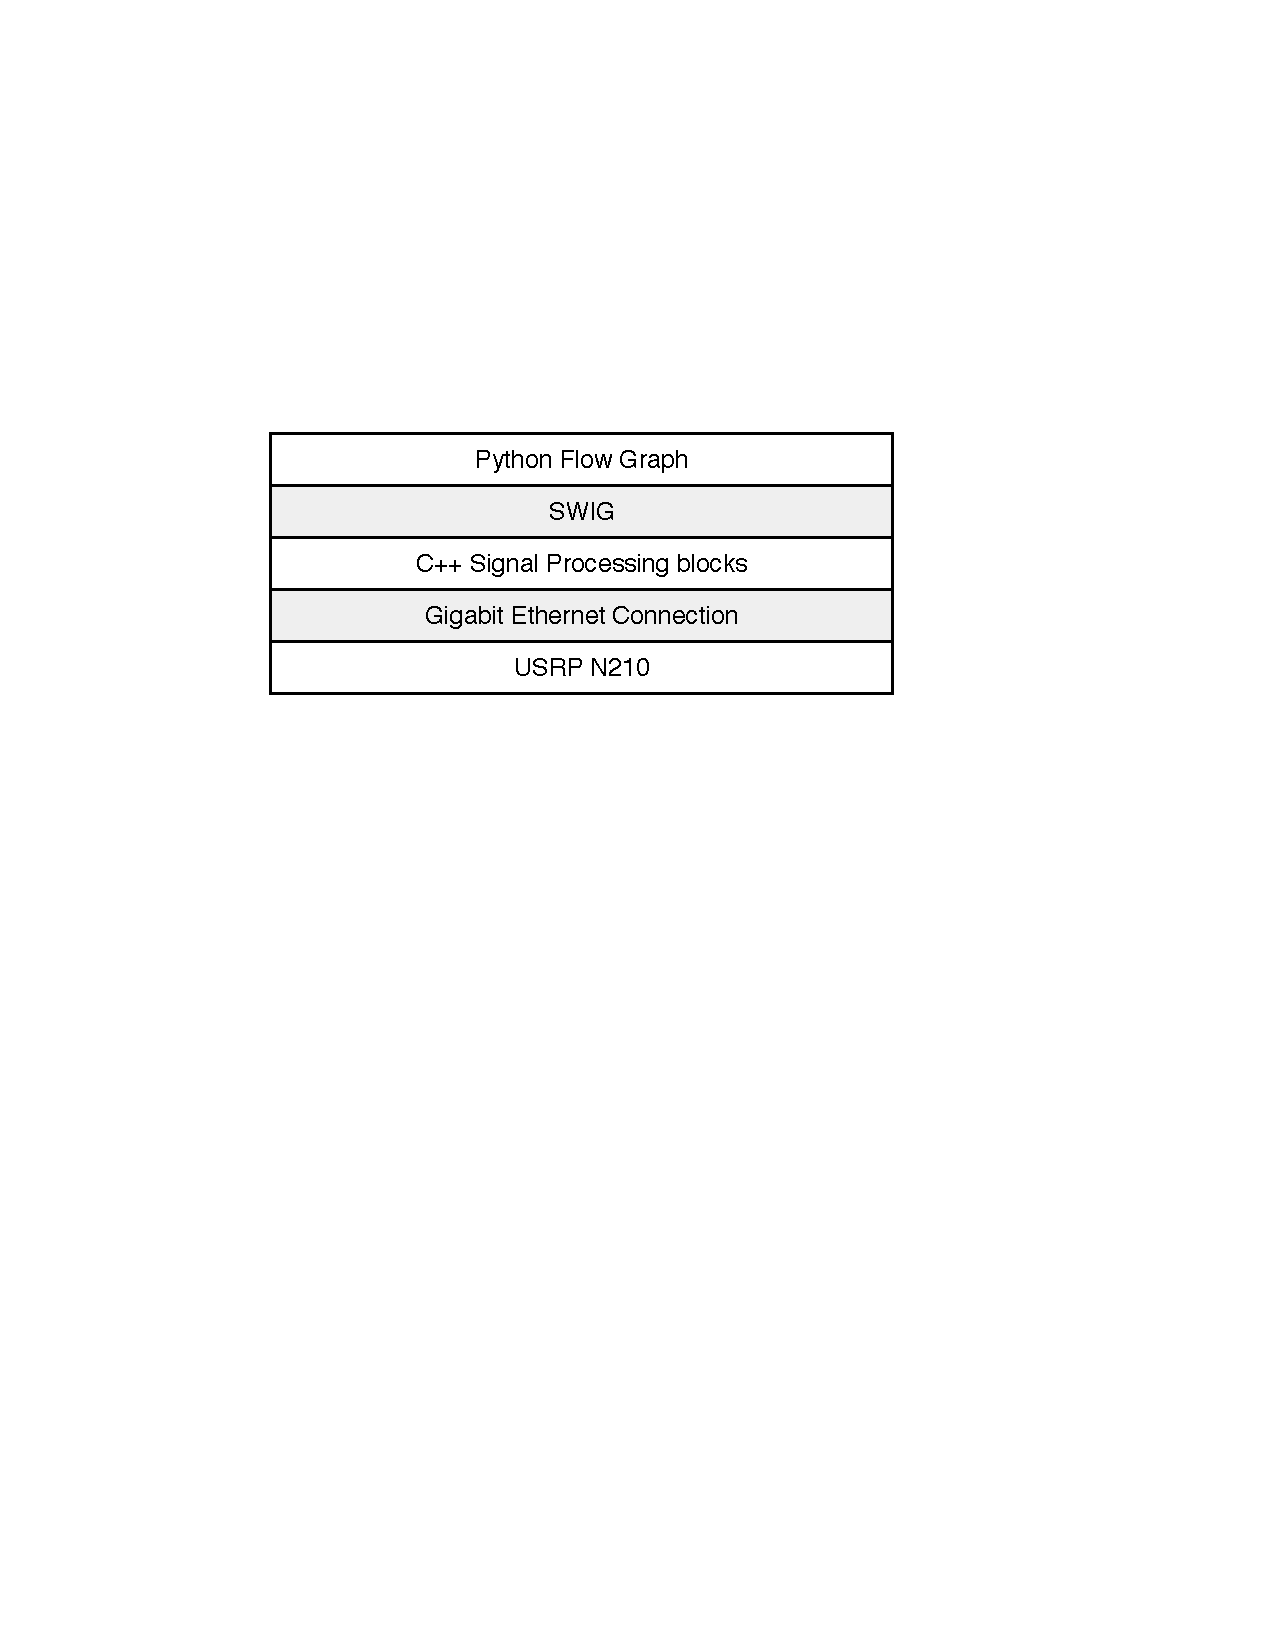
\includegraphics[width=1\textwidth]{gnuradio_architecture}
\caption{Architecture of GNU Radio}
\label{gnuradio_architecture}
\end{figure}

The USRP and the host computer make up the hardware part of the SDR system. The host computer must run a compatible software package such as GNU Radio or Simulink to complete the SDR system. In this project we are using GNU Radio as the software platform.

GNU Radio communicates with the USRP through the USRP Hardware Driver (UHD) software. The UHD provides a host driver and an Application Programming Interface (API) for the USRP. GNU Radio uses the UHD to set user-specified parameters like RF center frequency, antenna selection, gain, sampling rate, interpolation, decimation, etc.

\chapter{OpenBTS}

\section{What is OpenBTS?}
OpenBTS is a Unix application that uses a software radio to present a GSM Um interface to handsets and uses a SIP softswitch or PBX to connect calls.(You might even say that OpenBTS is a simplified form of IMS that works with 2G feature-phone handsets). The combination of the global -standard GSM air interface with low cost VoIP backhaul forms the basis of a new type of cellular network that can be deployed and operated at substantially lower cost than existing technologies in many applications, especially rural cellular deployments and private cellular networks in remote areas.

\section{The OpenBTS Application Suite}
A complete OpenBTS P2.8 installation comprises several distinct applications:

\begin{description}
	\item[OpenBTS] The actual OpenBTS application, containing most of the GSM stack above the radio modem.
	\item[Transceiver] The software radio modem and hardware control interface.
	\item[Asterisk] The VoIP PBX in the standard public release configuration.
	\item[Smqueue] The store-and-forward server for text messaging.
	\item[Subscriber Registry] A database of subscriber information that replaces both the Asterisk SIP registry and the GSM Home Location Register (HLR).
	\item[Other Servers] Other optional GSM services, beyond speech and text messaging, are supported through external servers.
\end{description}

The OpenBTS and Transceiver applications must run inside each GSM/SIP access point. The Asterisk and the subscriber registry applications communicated through the filesystem and therefore must run on the same computer, but that computer can be remote from the access point. smqueue and the other servers can run anywhere and may have multiple instances.

 \subsection{OpenBTS}
The OpenBTS application contains:
\begin{itemize}
	\item L1 Time division multiplexing(TDM) functions (GSM 05.02)
	\item L1 Forward error correction(FEC) functions (GSM 05.03)
	\item L1 closed loop power and timing controls (GSM 05.08 and 05.10)
	\item L2 Link access protocol on Dm-channel (LAPDm)  (GSM 04.06)
	\item L3 radio resource management functions (GSM 04.08)
	\item L3 GSM-SIP gateway for mobility management
	\item L3 GSM-SIP gateway for call control
	\item L4 GSM-SIP gateway for text messaging
\end{itemize}

The general design approach of OpenBTS is avoid implementing any function above L3, so at L3 or L4 every subprotocol of GSM is either terminated locally or translated through a gateway to some other protocol for handling by an external application. Similarly, OpenBTS itself does not contain any speech transcoding functions above the L1 FEC parts.

\subsection{Transceiver}
The transceiver application performs the radio modem functions of GSM 05.05 and manages the Gigabit Ethernet interface
(USB2 interface, in case
of USRP1 or older models) to the radio hardware.

\subsection{Asterisk}
OpenBTS uses a SIP switch or PBX to perform the call control functions that would normally be performed by the mobile switching center in a conventional GSM network, although in most network configurations this switching function is distributed over multiple switches. These switches also provide transcoding services. In OpenBTS P2.8 the standard SIP switch is Asterisk 1.8.

\subsection{Subscriber Registry}
OpenBTS uses a modified SIP registry as a substitute for the home location register found in a conventional GSM network. OpenBTS also relies on Asterisk for any transcoding functions. 

\subsection{Smqueue}
Smqueue is a store-and-forward server that is used for text messaging in the OpenBTS system. Smqueue is required to send a text message from one MS to another, or to provide reliable delivery of text messages to an MS from any source.

\subsection{Network Organization}
In the simplest network, with a single access point, all of the applications in the suite run inside the access point on the same embedded computer.



\begin{figure}[h]
\centering
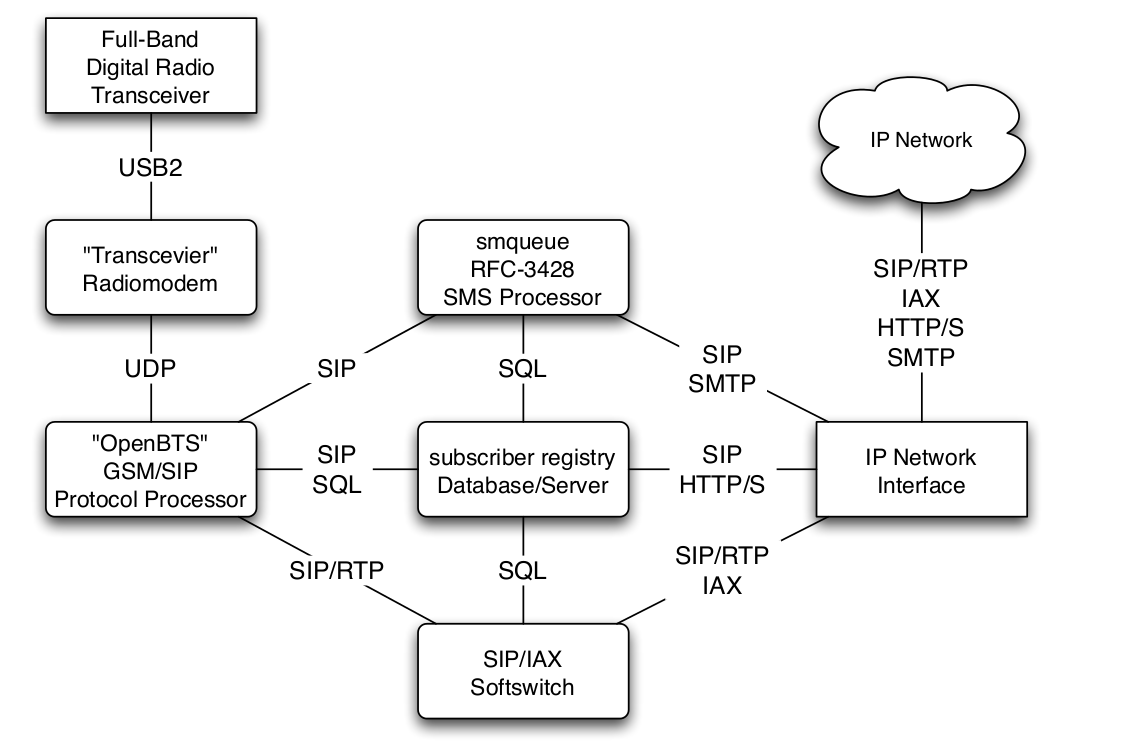
\includegraphics[width=1\textwidth]{networkOrg}
\caption{\textbf{Network Organization of OpenBTS}: The smqueue block handles SMSs. 
The subscriber registry database contains the details of all registered users and it
maps the registered IMSIs to corresponding dialling numbers. The softswitch connects 
speech calls (e.g. Asterisk, FreeSwitch). The transceiver performs radio modem
functions and manages the Gigabit Ethernet interface (USB2 interface, in case
of USRP1 or older models) to the USRP device. The OpenBTS itself is the GSM 
implementation from the TDMA part of L1 up through L3 and the L3/L4 boundary. 
It has a SIP interface to communicate with the other blocks like smqueue, subscriber 
registry, etc.
}
\label{networkOrg}
\end{figure}





















\chapter{OpenBTS with a cognitive approach}


\section{Target}

Our goal is to set up an OpenBTS system with cognitive capabilities. We decide on a frequency channel, to run our cognitive OpenBTS system in, beforehand. First we sense the presence of ongoing calls made by primary users in the predefined frequency channel. If there are ongoing calls in that channel then we wait for the calls to end. As soon as the calls made by primary users end, we start our secondary OpenBTS system to allow secondary users to make calls.

\section{Spectrum Sensing}

Spectrum sensing is the task of finding spectrum holes (or empty spectrum) in the local neighborhood of the cognitive radio receiver. Spectrum holes are the empty or unused portions of the spectrum at a particular space and time. Spectrum sensing lies at the very heart of cognitive radio technology. Cognitive radio works by utilizing the unused portions of the spectrum and for this to be possible, we need to find those empty portions of the spectrum at the very first. 

Detecting the presence of primary users is considered the most efficient way of spectrum sensing. Some of the ways to detect primary users are:

\begin{itemize}
	\item Energy detection
	\item Matched filter detection
	\item Cyclostationary detection
\end{itemize}

\subsection{Energy Detection}

This method of detecting primary users is the simplest one. It requires no a-priori knowledge about the signal to be detected. Basically the energy of the frequency band in question is calculated and compared to a predefined threshold to determine whether a primary user is present in that frequency band or not. Energy detection is simple to implement and relatively not so expensive in terms of required computing resources.
This method is not without disadvantages. Firstly deciding on a good threshold energy level is difficult. It cannot differentiate between primary users and secondary users. At low SNR, distinguishing a signal from noise is difficult. Averaging out the noise by using longer observation period can also lead to inefficient use of time. 

figure page 17




figure gives block diagram to implement the energy detection using the periodogram method. Spectrum sensing is a binary hypothesis testing problem with tow possible hypothesis $H0$ and $H1$. The hypothesis $H0$ defines that there is no PU present and hypothesis $H1$ defines that there is a PU present. The goal of energy detection is to distinguish between these two hypothesis[6]:

\begin{align}
	x(t) &= n(t), \qquad & H0 \nonumber\\
		&= h s(t)+n(t), \qquad & H1 \nonumber
\end{align}

where $x(t)$ is signal received by secondary user and $s(t)$ is signal transmitted by primary user, $n(t)$ is additive white Gaussian noise (AWGN) and $h$ is the amplitude gain of the channel. It is assumed that $s(t)$  and $n(t)$ are independent of each other. Signal detection is performed using an energy detector and compute decision statistics $Y$ which corresponds to energy collected in observation time $Y$ and bandwidth $W$ and comparing this statistics to a predetermined threshold. 

.
\subsubsection{Average Periodogram Analysis}
 It is technique used as an energy detection method for determining the presence or absence of primary traffic. 
Power spectrum is estimated using periodogram analysis, which is based on discrete fourier transform (DFT) of finite length segments of signal. It involves sectioning the data into finite segments to compute individual periodogram or modified periodogram and averaging the modified periodogram segments.


Let $X[n], n=0,1,...,L-$1 be the discrete time signal that are divided into $K$ finite length equal segments, where length of each segment is $N$ i.e. $KN = L; Xr[n], n= 0,1,..., N-1$ is the $r$th segment and $W[n], n=0,1,...,N-1$ be the window applied to each segment. The modified periodogram for the $r$th segment is,

\begin{equation*}
	I_{r}[k] = \frac{1}{NU}\vert{}V_{r}[k]\vert{}^2     \qquad k=0,1,...,N-1
\end{equation*}

where $V_{r}[k]$ is a $N$ point DFT and $U$ is normalization factor i.e. ,
$V_{r}[k] = DFT\{W[n]*X[n]\}$  and 
$U = \frac{1}{N}(\sum_{n=0}^{N-1}(W[n])^2)$.


The PSD of $X[n]$ sequence or the time averaged periodogram estimate ,
\begin{equation*}
\bar{I}[k] = \frac{1}{K}\sum_{r=0}^{K-1}Ir[k]
\end{equation*}

One of the most relevant tools for wide band spectrum sensing is GNU radio spectrum sensor \mbox{``usrp\_spectrum\_sense.py''.}
 This program can be used as a basic code for implementing wideband spectrum analyzer. The output is  $Y[i] = re[X[i]]*re[X[i]] + im[X[i]]*im[X[i]]$.
To use $N$ point complex FFT $X(W)$ analysis, we have to get $N$ time samples of $x(t)$  which are sampled at $Fs$. These time samples must be time windowed using a known window function to reduce spectral leakage. The output of the complex FFT will represent the frequency spectrum content as follows:
The first value of the FFT output ($bin 0 == X[0]$) is the passband centre frequency
The first half of FFT spectrum ($X[1]$ to $X[N/2-1]$) contains the positive baseband frequencies, which corresponds to the passband spectrum from centre frequency to $+Fs/2$.
The second half of the FFT ($X[N/2]$ to $X[N-1$]) contains the negative baseband frequencies, i.e. from $-Fs/2$ to centre frequency.


In our case bla bla aur scenario����������������

SETUP 

fig 









 The above figure describes the whole setup that we have used for our project 

 ...description of the set up�����..
 
We have been able to successfully sense the presence of primary user in the predefined frequency band and as soon as the primary user leaves the energy in that band goes low and we are able to switch on the secondary BTS and secondary users are able to make calls and transmit SMS�s using secondary BTS. 

We have also been able write python script to kill all the four processes of openBTS. Also we are able to connect two USRP kits on the same computer and run GNURadio and OpenBTS parallelly which we were not able to initially. GNU Radio will be used to continuously sense the spectrum to identify the presence of primary user and provide the optimum ARFCN for OpenBTS to start. 

What we aim to achieve is after GNUradio has provided particular ARFCN corresponding to certain frequency (say F1) to OpenBTS, it will continue sensing for primary users in this frequency on which OpenBTS is currently operating and if it finds that the energy in that frequency goes above some predefined threshold then secondary OpenBTS will close thus avoiding interference to primary users and it restart on another frequency(say F2). Now GNURadio will look for primary users in this frequency F2 by checking if the energy in this frequency is going beyond some predefined threshold.

 
The following flow graph summerizes what we aim to achieve.




 


%\chapter{Spectrum Sensing}
\section{Matched filter detection}
\section{Energy based detection}
%\chapter{A cognitive base station using GnuRadio and OpenBTS}
\section{Motivation}



\appendix
\chapter{Codes}

\section{senseUplinknStartBTS.py}

\begin{lstlisting}[language=Python]

#!/usr/bin/env python
#
# Copyright 2005,2007,2011 Free Software Foundation, Inc.
#
# This file is part of GNU Radio
#
# GNU Radio is free software; you can redistribute it and/or modify
# it under the terms of the GNU General Public License as published by
# the Free Software Foundation; either version 3, or (at your option)
# any later version.
#
# GNU Radio is distributed in the hope that it will be useful,
# but WITHOUT ANY WARRANTY; without even the implied warranty of
# MERCHANTABILITY or FITNESS FOR A PARTICULAR PURPOSE.  See the
# GNU General Public License for more details.
#
# You should have received a copy of the GNU General Public License
# along with GNU Radio; see the file COPYING.  If not, write to
# the Free Software Foundation, Inc., 51 Franklin Street,
# Boston, MA 02110-1301, USA.
#

from gnuradio import gr, eng_notation
from gnuradio import blocks
from gnuradio import audio
from gnuradio import filter
from gnuradio import fft
from gnuradio import uhd
from gnuradio.eng_option import eng_option
from optparse import OptionParser
import sys
import math
import struct
import threading
import time
import sqlite3
import os
import subprocess
from datetime import datetime

sys.stderr.write("Warning: this may have issues on some machines+Python version combinations to seg fault due to the callback in bin_statitics.\n\n")

class ThreadClass(threading.Thread):
    def run(self):
        return

class tune(gr.feval_dd):
    """
    This class allows C++ code to callback into python.
    """
    def __init__(self, tb):
        gr.feval_dd.__init__(self)
        self.tb = tb

    def eval(self, ignore):
        """
        This method is called from blocks.bin_statistics_f when it wants
        to change the center frequency.  This method tunes the front
        end to the new center frequency, and returns the new frequency
        as its result.
        """

        try:
            # We use this try block so that if something goes wrong
            # from here down, at least we'll have a prayer of knowing
            # what went wrong.  Without this, you get a very
            # mysterious:
            #
            #   terminate called after throwing an instance of
            #   'Swig::DirectorMethodException' Aborted
            #
            # message on stderr.  Not exactly helpful ;)

            new_freq = self.tb.set_next_freq()
            
            # wait until msgq is empty before continuing
            while(self.tb.msgq.full_p()):
                #print "msgq full, holding.."
                time.sleep(0.1)
            
            return new_freq

        except Exception, e:
            print "tune: Exception: ", e


class parse_msg(object):
    def __init__(self, msg):
        self.center_freq = msg.arg1()
        self.vlen = int(msg.arg2())
        assert(msg.length() == self.vlen * gr.sizeof_float)

        # FIXME consider using NumPy array
        t = msg.to_string()
        self.raw_data = t
        self.data = struct.unpack('%df' % (self.vlen,), t)


class my_top_block(gr.top_block):

    def __init__(self):
        gr.top_block.__init__(self)

        usage = "usage: %prog [options] down_freq"
        parser = OptionParser(option_class=eng_option, usage=usage)
        parser.add_option("-a", "--args", type="string", default="",
                          help="UHD device device address args [default=%default]")
        parser.add_option("", "--spec", type="string", default=None,
	                  help="Subdevice of UHD device where appropriate")
        parser.add_option("-A", "--antenna", type="string", default=None,
                          help="select Rx Antenna where appropriate")
        parser.add_option("-s", "--samp-rate", type="eng_float", default=10e6,
                          help="set sample rate [default=%default]")
        parser.add_option("-g", "--gain", type="eng_float", default=None,
                          help="set gain in dB (default is midpoint)")
        parser.add_option("", "--tune-delay", type="eng_float",
                          default=0.25, metavar="SECS",
                          help="time to delay (in seconds) after changing frequency [default=%default]")
        parser.add_option("", "--dwell-delay", type="eng_float",
                          default=0.25, metavar="SECS",
                          help="time to dwell (in seconds) at a given frequency [default=%default]")
        parser.add_option("-b", "--channel-bandwidth", type="eng_float",
                          default=9.7656e3, metavar="Hz",
                          help="channel bandwidth of fft bins in Hz [default=%default]")
        parser.add_option("-l", "--lo-offset", type="eng_float",
                          default=0, metavar="Hz",
                          help="lo_offset in Hz [default=%default]")
        parser.add_option("-q", "--squelch-threshold", type="eng_float",
                          default=None, metavar="dB",
                          help="squelch threshold in dB [default=%default]")
        parser.add_option("-F", "--fft-size", type="int", default=None,
                          help="specify number of FFT bins [default=samp_rate/channel_bw]")
        parser.add_option("", "--real-time", action="store_true", default=False,
                          help="Attempt to enable real-time scheduling")


        (options, args) = parser.parse_args()
        if len(args) != 1:
            parser.print_help()
            sys.exit(1)

        self.channel_bandwidth = options.channel_bandwidth

        self.down_freq = eng_notation.str_to_num(args[0])
        self.up_freq = self.down_freq - 45e6



        if not options.real_time:
            realtime = False
        else:
            # Attempt to enable realtime scheduling
            r = gr.enable_realtime_scheduling()
            if r == gr.RT_OK:
                realtime = True
            else:
                realtime = False
                print "Note: failed to enable realtime scheduling"

        # build graph
        self.u = uhd.usrp_source(device_addr=options.args,
                                 stream_args=uhd.stream_args('fc32'))

        # Set the subdevice spec
        if(options.spec):
            self.u.set_subdev_spec(options.spec, 0)

        # Set the antenna
        if(options.antenna):
            self.u.set_antenna(options.antenna, 0)
        
        self.u.set_samp_rate(options.samp_rate)

        self.usrp_rate = usrp_rate = self.u.get_samp_rate()
        
        self.lo_offset = options.lo_offset

        if options.fft_size is None:
            self.fft_size = int(self.usrp_rate/self.channel_bandwidth)
        else:
            self.fft_size = options.fft_size
        
        self.squelch_threshold = options.squelch_threshold
        
        s2v = blocks.stream_to_vector(gr.sizeof_gr_complex, self.fft_size)

        mywindow = filter.window.blackmanharris(self.fft_size)
        ffter = fft.fft_vcc(self.fft_size, True, mywindow, True)
        power = 0
        for tap in mywindow:
            power += tap*tap

        c2mag = blocks.complex_to_mag_squared(self.fft_size)


        tune_delay  = max(0, int(round(options.tune_delay * usrp_rate / self.fft_size)))  # in fft_frames
        dwell_delay = max(1, int(round(options.dwell_delay * usrp_rate / self.fft_size))) # in fft_frames

        self.msgq = gr.msg_queue(1)
        self._tune_callback = tune(self)        # hang on to this to keep it from being GC'd
        stats = blocks.bin_statistics_f(self.fft_size, self.msgq,
                                        self._tune_callback, tune_delay,
                                        dwell_delay)

        # FIXME leave out the log10 until we speed it up
	#self.connect(self.u, s2v, ffter, c2mag, log, stats)
	self.connect(self.u, s2v, ffter, c2mag, stats)

        if options.gain is None:
            # if no gain was specified, use the mid-point in dB
            g = self.u.get_gain_range()
            options.gain = float(g.start()+g.stop())/2.0

        self.set_gain(options.gain)
        print "gain =", options.gain

    def set_next_freq(self):
        target_freq = self.up_freq


        if not self.set_freq(target_freq):
            print "Failed to set frequency to", target_freq
            sys.exit(1)

        return target_freq


    def set_freq(self, target_freq):
        """
        Set the center frequency we're interested in.

        Args:
            target_freq: frequency in Hz
        @rypte: bool
        """
        
        r = self.u.set_center_freq(uhd.tune_request(target_freq, rf_freq=(target_freq + self.lo_offset),rf_freq_policy=uhd.tune_request.POLICY_MANUAL))
        if r:
            return True

        return False

    def set_gain(self, gain):
        self.u.set_gain(gain)
    


def main_loop(tb):
    
    # use a counter to make sure power is less than threshold
    lowPowerCount = 0
    lowPowerCountMax = 10
    print 'fft size', tb.fft_size
    N = tb.fft_size
    

    while 1:

        # Get the next message sent from the C++ code (blocking call).
        # It contains the center frequency and the mag squared of the fft
        m = parse_msg(tb.msgq.delete_head())

        # m.center_freq is the center frequency at the time of capture
        # m.data are the mag_squared of the fft output
        # m.raw_data is a string that contains the binary floats.
        # You could write this as binary to a file.



        center_freq = m.center_freq
        bins = 10
        power_data = 0
        
        for i in range(1, bins+1):
            power_data += m.data[N-i] + m.data[i]
        power_data += m.data[0]
        power_data /= ((2*bins) + 1)
        
        power_db = 10*math.log10(power_data/tb.usrp_rate)
        power_threshold = -95

        if (power_db > tb.squelch_threshold) and (power_db > power_threshold):
            print datetime.now(), "center_freq", center_freq, "power_db", power_db, "in use"
            lowPowerCount = 0
        else:
            print datetime.now(), "center_freq", center_freq, "power_db", power_db
            lowPowerCount += 1
            if (lowPowerCount > lowPowerCountMax):
                down_freq = center_freq + 45e6
                startOpenBTS(down_freq)
                break


def startOpenBTS(downFrequency):            
    
    
    arfcn=int((downFrequency-935e6)/2e5)
    if (arfcn < 0):
        print "ARFCN must be > 0 !!!"
        sys.exit(1)
    print 'ARFCN=', arfcn
    #DB modifications
    t=(arfcn,)
    conn=sqlite3.connect("/etc/OpenBTS/OpenBTS.db")
    cursor=conn.cursor()
    cursor.execute("update config set valuestring=? where keystring='GSM.Radio.C0'",t)
    conn.commit()

    #start the OpenBTS
    f=subprocess.Popen(os.path.expanduser('~/ddp-stage-1-and-openbts/runOpenBTS.sh'))
    f.wait()
	          

if __name__ == '__main__':
    t = ThreadClass()
    t.start()

    tb = my_top_block()
    try:
        tb.start()
        main_loop(tb)

    except KeyboardInterrupt:
        pass


\end{lstlisting}



\backmatter
\bibliographystyle{plain}
\bibliography{ddpStage1}

\end{document}